\documentclass[twoside]{book}

% Packages required by doxygen
\usepackage{fixltx2e}
\usepackage{calc}
\usepackage{doxygen}
\usepackage[export]{adjustbox} % also loads graphicx
\usepackage{graphicx}
\usepackage[utf8]{inputenc}
\usepackage{makeidx}
\usepackage{multicol}
\usepackage{multirow}
\PassOptionsToPackage{warn}{textcomp}
\usepackage{textcomp}
\usepackage[nointegrals]{wasysym}
\usepackage[table]{xcolor}

% Font selection
\usepackage[T1]{fontenc}
\usepackage[scaled=.90]{helvet}
\usepackage{courier}
\usepackage{amssymb}
\usepackage{sectsty}
\renewcommand{\familydefault}{\sfdefault}
\allsectionsfont{%
  \fontseries{bc}\selectfont%
  \color{darkgray}%
}
\renewcommand{\DoxyLabelFont}{%
  \fontseries{bc}\selectfont%
  \color{darkgray}%
}
\newcommand{\+}{\discretionary{\mbox{\scriptsize$\hookleftarrow$}}{}{}}

% Page & text layout
\usepackage{geometry}
\geometry{%
  a4paper,%
  top=2.5cm,%
  bottom=2.5cm,%
  left=2.5cm,%
  right=2.5cm%
}
\tolerance=750
\hfuzz=15pt
\hbadness=750
\setlength{\emergencystretch}{15pt}
\setlength{\parindent}{0cm}
\setlength{\parskip}{3ex plus 2ex minus 2ex}
\makeatletter
\renewcommand{\paragraph}{%
  \@startsection{paragraph}{4}{0ex}{-1.0ex}{1.0ex}{%
    \normalfont\normalsize\bfseries\SS@parafont%
  }%
}
\renewcommand{\subparagraph}{%
  \@startsection{subparagraph}{5}{0ex}{-1.0ex}{1.0ex}{%
    \normalfont\normalsize\bfseries\SS@subparafont%
  }%
}
\makeatother

% Headers & footers
\usepackage{fancyhdr}
\pagestyle{fancyplain}
\fancyhead[LE]{\fancyplain{}{\bfseries\thepage}}
\fancyhead[CE]{\fancyplain{}{}}
\fancyhead[RE]{\fancyplain{}{\bfseries\leftmark}}
\fancyhead[LO]{\fancyplain{}{\bfseries\rightmark}}
\fancyhead[CO]{\fancyplain{}{}}
\fancyhead[RO]{\fancyplain{}{\bfseries\thepage}}
\fancyfoot[LE]{\fancyplain{}{}}
\fancyfoot[CE]{\fancyplain{}{}}
\fancyfoot[RE]{\fancyplain{}{\bfseries\scriptsize Generated by Doxygen }}
\fancyfoot[LO]{\fancyplain{}{\bfseries\scriptsize Generated by Doxygen }}
\fancyfoot[CO]{\fancyplain{}{}}
\fancyfoot[RO]{\fancyplain{}{}}
\renewcommand{\footrulewidth}{0.4pt}
\renewcommand{\chaptermark}[1]{%
  \markboth{#1}{}%
}
\renewcommand{\sectionmark}[1]{%
  \markright{\thesection\ #1}%
}

% Indices & bibliography
\usepackage{natbib}
\usepackage[titles]{tocloft}
\setcounter{tocdepth}{3}
\setcounter{secnumdepth}{5}
\makeindex

% Hyperlinks (required, but should be loaded last)
\usepackage{ifpdf}
\ifpdf
  \usepackage[pdftex,pagebackref=true]{hyperref}
\else
  \usepackage[ps2pdf,pagebackref=true]{hyperref}
\fi
\hypersetup{%
  colorlinks=true,%
  linkcolor=blue,%
  citecolor=blue,%
  unicode%
}

% Custom commands
\newcommand{\clearemptydoublepage}{%
  \newpage{\pagestyle{empty}\cleardoublepage}%
}

\usepackage{caption}
\captionsetup{labelsep=space,justification=centering,font={bf},singlelinecheck=off,skip=4pt,position=top}

%===== C O N T E N T S =====

\begin{document}

% Titlepage & ToC
\hypersetup{pageanchor=false,
             bookmarksnumbered=true,
             pdfencoding=unicode
            }
\pagenumbering{alph}
\begin{titlepage}
\vspace*{7cm}
\begin{center}%
{\Large My Project }\\
\vspace*{1cm}
{\large Generated by Doxygen 1.8.13}\\
\end{center}
\end{titlepage}
\clearemptydoublepage
\pagenumbering{roman}
\tableofcontents
\clearemptydoublepage
\pagenumbering{arabic}
\hypersetup{pageanchor=true}

%--- Begin generated contents ---
\chapter{Li2}
\label{md_README}
\Hypertarget{md_README}
Alunos esses que pertence ao P\+L1-\/\+Grupo 2, sendo eles\+:

Pedro Aquino Martins de Araujo-\/ A90614

Pedro Henrique do Vale Saldanha-\/ A90618

Vitor Lelis Noronha Leite-\/ A90707 
\chapter{relatorio}
\label{md_relatorio}
\Hypertarget{md_relatorio}
M\+I\+E\+I-\/\+UC 1º ano-\/2º S\+E\+M\+E\+S\+T\+RE Numeração do grupo\+:2 P\+L1 Grupo\+: Pedro Aquino A90614 Pedro Saldanha A90618 Vitor Lelis A90707

Relatorio (Guião 5)

Objetivo\+:Neste guião tivemos como tarefa produzir modulos, além de desenvolver código para cada modulo sendo eles (Camada\+De\+Dados,logica, interface).

Desafios\+: Nas primeiras impressões o código de exemplo parecia ser demasiado complexo pelo facto de utilizar algumas funções não apresentadas ou estudadas em sala de aula,com isso,foi preciso sentar os três a tentar analisar o código que vos foi dado, além disso, tivemos uma discursão o que seria melhor para o desenvolvimento do trabalho,fazer o nosso próprio código ou utilizar os ja estava pre estabelecido.\+Sendo assim, depois de 3 dias de analise de código para percebemos o que cada função faz, começamos a reparar o como as partes se encaixavam de forma simples e clara e então inicializamos o nosso desenvolvimento. Diante disto, ficamos um pouco perdidos em relação o que tínhamos que complementar e como poderíamos construir um código para que ficasse tão compacto e simples como o já estabelecido.\+Embora,apesar nos apresentar um código que é simples nos faltava conhecimento mas conseguimos aprender um pouco mais das funções e com os nossos erros em testes. 
\chapter{Class Index}
\section{Class List}
Here are the classes, structs, unions and interfaces with brief descriptions\+:\begin{DoxyCompactList}
\item\contentsline{section}{\hyperlink{structCOORDENADA}{C\+O\+O\+R\+D\+E\+N\+A\+DA} }{\pageref{structCOORDENADA}}{}
\item\contentsline{section}{\hyperlink{structESTADO}{E\+S\+T\+A\+DO} }{\pageref{structESTADO}}{}
\item\contentsline{section}{\hyperlink{structJOGADA}{J\+O\+G\+A\+DA} }{\pageref{structJOGADA}}{}
\end{DoxyCompactList}

\chapter{Class Documentation}
\hypertarget{structCOORDENADA}{}\section{C\+O\+O\+R\+D\+E\+N\+A\+DA Struct Reference}
\label{structCOORDENADA}\index{C\+O\+O\+R\+D\+E\+N\+A\+DA@{C\+O\+O\+R\+D\+E\+N\+A\+DA}}


{\ttfamily \#include $<$camada\+De\+Dados.\+h$>$}

\subsection*{Public Attributes}
\begin{DoxyCompactItemize}
\item 
\mbox{\Hypertarget{structCOORDENADA_acb526f8ae91ba6a2742ef1a9473fa2b4}\label{structCOORDENADA_acb526f8ae91ba6a2742ef1a9473fa2b4}} 
int {\bfseries letra}
\item 
\mbox{\Hypertarget{structCOORDENADA_aefe14bcc5a066ac3b21500cc3d28c06f}\label{structCOORDENADA_aefe14bcc5a066ac3b21500cc3d28c06f}} 
int {\bfseries linha}
\item 
\mbox{\Hypertarget{structCOORDENADA_ac00ff2e615b371a3d87fbb05449cde99}\label{structCOORDENADA_ac00ff2e615b371a3d87fbb05449cde99}} 
char {\bfseries letrinha}
\end{DoxyCompactItemize}


\subsection{Detailed Description}
\hyperlink{structCOORDENADA}{C\+O\+O\+R\+D\+E\+N\+A\+DA} há dois inteiros sendo eles para identificar as colunas=letras (A-\/H),linhas de (1-\/8) e o letrinh é um char para utilizamos no movs e prompt . 
\begin{DoxyParams}{Parameters}
{\em letra} & é a coordenada das colunas \\
\hline
\end{DoxyParams}


The documentation for this struct was generated from the following file\+:\begin{DoxyCompactItemize}
\item 
camada\+De\+Dados.\+h\end{DoxyCompactItemize}

\hypertarget{structESTADO}{}\section{E\+S\+T\+A\+DO Struct Reference}
\label{structESTADO}\index{E\+S\+T\+A\+DO@{E\+S\+T\+A\+DO}}


Informações do estado tab(tabuleiro), numero de jogadas (começa no 0), jogador atual (começa no jogador 1)  




{\ttfamily \#include $<$camada\+De\+Dados.\+h$>$}



Collaboration diagram for E\+S\+T\+A\+DO\+:\nopagebreak
\begin{figure}[H]
\begin{center}
\leavevmode
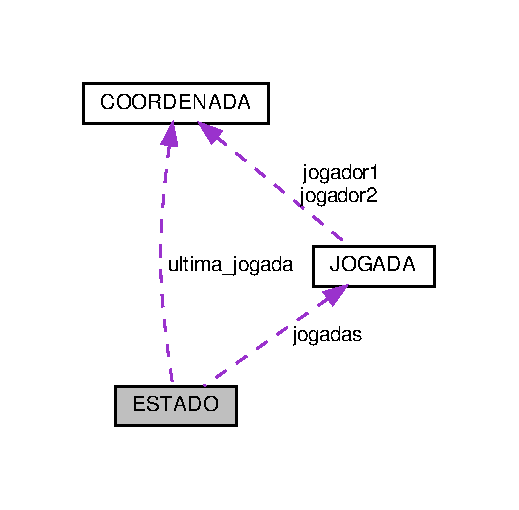
\includegraphics[width=249pt]{structESTADO__coll__graph}
\end{center}
\end{figure}
\subsection*{Public Attributes}
\begin{DoxyCompactItemize}
\item 
C\+A\+SA \hyperlink{structESTADO_ab56f0f1be16954d3768b4174d14c087d}{tab} \mbox{[}8\mbox{]}\mbox{[}8\mbox{]}
\item 
J\+O\+G\+A\+D\+AS \hyperlink{structESTADO_afae43b87a488fad0f2b56a18bad31d18}{jogadas}
\item 
int \hyperlink{structESTADO_a261495728744647e618b4e623f5a4b7a}{num\+\_\+jogadas}
\item 
int \hyperlink{structESTADO_a5dd28e2e68b7aef2b6b7ea88e02eff58}{jogador\+\_\+atual}
\item 
int \hyperlink{structESTADO_a5632721fdfcc6c98f084c91aef5b6e25}{count\+\_\+jog}
\item 
int \hyperlink{structESTADO_a36e8d21ac156e82ce914ccdafc6796ea}{count\+\_\+mov}
\item 
int \hyperlink{structESTADO_a49b04d6940f820509146c9162ac10542}{count\+\_\+movs}
\item 
int \hyperlink{structESTADO_a248a8554633b7e8e40142e5b8c4e6960}{num}
\item 
int \hyperlink{structESTADO_ae0aaae1dc17799598305cd40a3ca2ba8}{qntjogs}
\item 
\hyperlink{structCOORDENADA}{C\+O\+O\+R\+D\+E\+N\+A\+DA} \hyperlink{structESTADO_ab9b11998a54bde459f72cbbc32e79b0b}{possiveis\+\_\+jog} \mbox{[}8\mbox{]}
\item 
\hyperlink{structCOORDENADA}{C\+O\+O\+R\+D\+E\+N\+A\+DA} \hyperlink{structESTADO_a4896a5c5c1f40b43fb795623327e3f47}{ultima\+\_\+jogada}
\end{DoxyCompactItemize}


\subsection{Detailed Description}
Informações do estado tab(tabuleiro), numero de jogadas (começa no 0), jogador atual (começa no jogador 1) 

\subsection{Member Data Documentation}
\mbox{\Hypertarget{structESTADO_a5632721fdfcc6c98f084c91aef5b6e25}\label{structESTADO_a5632721fdfcc6c98f084c91aef5b6e25}} 
\index{E\+S\+T\+A\+DO@{E\+S\+T\+A\+DO}!count\+\_\+jog@{count\+\_\+jog}}
\index{count\+\_\+jog@{count\+\_\+jog}!E\+S\+T\+A\+DO@{E\+S\+T\+A\+DO}}
\subsubsection{\texorpdfstring{count\+\_\+jog}{count\_jog}}
{\footnotesize\ttfamily int E\+S\+T\+A\+D\+O\+::count\+\_\+jog}

Contador para a troca de jogador \mbox{\Hypertarget{structESTADO_a36e8d21ac156e82ce914ccdafc6796ea}\label{structESTADO_a36e8d21ac156e82ce914ccdafc6796ea}} 
\index{E\+S\+T\+A\+DO@{E\+S\+T\+A\+DO}!count\+\_\+mov@{count\+\_\+mov}}
\index{count\+\_\+mov@{count\+\_\+mov}!E\+S\+T\+A\+DO@{E\+S\+T\+A\+DO}}
\subsubsection{\texorpdfstring{count\+\_\+mov}{count\_mov}}
{\footnotesize\ttfamily int E\+S\+T\+A\+D\+O\+::count\+\_\+mov}

Contador para todos os movimentos do jogo \mbox{\Hypertarget{structESTADO_a49b04d6940f820509146c9162ac10542}\label{structESTADO_a49b04d6940f820509146c9162ac10542}} 
\index{E\+S\+T\+A\+DO@{E\+S\+T\+A\+DO}!count\+\_\+movs@{count\+\_\+movs}}
\index{count\+\_\+movs@{count\+\_\+movs}!E\+S\+T\+A\+DO@{E\+S\+T\+A\+DO}}
\subsubsection{\texorpdfstring{count\+\_\+movs}{count\_movs}}
{\footnotesize\ttfamily int E\+S\+T\+A\+D\+O\+::count\+\_\+movs}

Contador para os movimentos sendo auxiliar para a funcionalidade do estado \mbox{\Hypertarget{structESTADO_afae43b87a488fad0f2b56a18bad31d18}\label{structESTADO_afae43b87a488fad0f2b56a18bad31d18}} 
\index{E\+S\+T\+A\+DO@{E\+S\+T\+A\+DO}!jogadas@{jogadas}}
\index{jogadas@{jogadas}!E\+S\+T\+A\+DO@{E\+S\+T\+A\+DO}}
\subsubsection{\texorpdfstring{jogadas}{jogadas}}
{\footnotesize\ttfamily J\+O\+G\+A\+D\+AS E\+S\+T\+A\+D\+O\+::jogadas}

Array conte todas as jogadas feitas \mbox{\Hypertarget{structESTADO_a5dd28e2e68b7aef2b6b7ea88e02eff58}\label{structESTADO_a5dd28e2e68b7aef2b6b7ea88e02eff58}} 
\index{E\+S\+T\+A\+DO@{E\+S\+T\+A\+DO}!jogador\+\_\+atual@{jogador\+\_\+atual}}
\index{jogador\+\_\+atual@{jogador\+\_\+atual}!E\+S\+T\+A\+DO@{E\+S\+T\+A\+DO}}
\subsubsection{\texorpdfstring{jogador\+\_\+atual}{jogador\_atual}}
{\footnotesize\ttfamily int E\+S\+T\+A\+D\+O\+::jogador\+\_\+atual}

Jogador atual \mbox{\Hypertarget{structESTADO_a248a8554633b7e8e40142e5b8c4e6960}\label{structESTADO_a248a8554633b7e8e40142e5b8c4e6960}} 
\index{E\+S\+T\+A\+DO@{E\+S\+T\+A\+DO}!num@{num}}
\index{num@{num}!E\+S\+T\+A\+DO@{E\+S\+T\+A\+DO}}
\subsubsection{\texorpdfstring{num}{num}}
{\footnotesize\ttfamily int E\+S\+T\+A\+D\+O\+::num}

Caso de paragem \mbox{\Hypertarget{structESTADO_a261495728744647e618b4e623f5a4b7a}\label{structESTADO_a261495728744647e618b4e623f5a4b7a}} 
\index{E\+S\+T\+A\+DO@{E\+S\+T\+A\+DO}!num\+\_\+jogadas@{num\+\_\+jogadas}}
\index{num\+\_\+jogadas@{num\+\_\+jogadas}!E\+S\+T\+A\+DO@{E\+S\+T\+A\+DO}}
\subsubsection{\texorpdfstring{num\+\_\+jogadas}{num\_jogadas}}
{\footnotesize\ttfamily int E\+S\+T\+A\+D\+O\+::num\+\_\+jogadas}

Numero de jogadas \mbox{\Hypertarget{structESTADO_ab9b11998a54bde459f72cbbc32e79b0b}\label{structESTADO_ab9b11998a54bde459f72cbbc32e79b0b}} 
\index{E\+S\+T\+A\+DO@{E\+S\+T\+A\+DO}!possiveis\+\_\+jog@{possiveis\+\_\+jog}}
\index{possiveis\+\_\+jog@{possiveis\+\_\+jog}!E\+S\+T\+A\+DO@{E\+S\+T\+A\+DO}}
\subsubsection{\texorpdfstring{possiveis\+\_\+jog}{possiveis\_jog}}
{\footnotesize\ttfamily \hyperlink{structCOORDENADA}{C\+O\+O\+R\+D\+E\+N\+A\+DA} E\+S\+T\+A\+D\+O\+::possiveis\+\_\+jog\mbox{[}8\mbox{]}}

Array com as possiveis coordenadas \mbox{\Hypertarget{structESTADO_ae0aaae1dc17799598305cd40a3ca2ba8}\label{structESTADO_ae0aaae1dc17799598305cd40a3ca2ba8}} 
\index{E\+S\+T\+A\+DO@{E\+S\+T\+A\+DO}!qntjogs@{qntjogs}}
\index{qntjogs@{qntjogs}!E\+S\+T\+A\+DO@{E\+S\+T\+A\+DO}}
\subsubsection{\texorpdfstring{qntjogs}{qntjogs}}
{\footnotesize\ttfamily int E\+S\+T\+A\+D\+O\+::qntjogs}

Conta quantas possiveis jogadas \mbox{\Hypertarget{structESTADO_ab56f0f1be16954d3768b4174d14c087d}\label{structESTADO_ab56f0f1be16954d3768b4174d14c087d}} 
\index{E\+S\+T\+A\+DO@{E\+S\+T\+A\+DO}!tab@{tab}}
\index{tab@{tab}!E\+S\+T\+A\+DO@{E\+S\+T\+A\+DO}}
\subsubsection{\texorpdfstring{tab}{tab}}
{\footnotesize\ttfamily C\+A\+SA E\+S\+T\+A\+D\+O\+::tab\mbox{[}8\mbox{]}\mbox{[}8\mbox{]}}

Tabuleiro no qual realizamos as jogadas \mbox{\Hypertarget{structESTADO_a4896a5c5c1f40b43fb795623327e3f47}\label{structESTADO_a4896a5c5c1f40b43fb795623327e3f47}} 
\index{E\+S\+T\+A\+DO@{E\+S\+T\+A\+DO}!ultima\+\_\+jogada@{ultima\+\_\+jogada}}
\index{ultima\+\_\+jogada@{ultima\+\_\+jogada}!E\+S\+T\+A\+DO@{E\+S\+T\+A\+DO}}
\subsubsection{\texorpdfstring{ultima\+\_\+jogada}{ultima\_jogada}}
{\footnotesize\ttfamily \hyperlink{structCOORDENADA}{C\+O\+O\+R\+D\+E\+N\+A\+DA} E\+S\+T\+A\+D\+O\+::ultima\+\_\+jogada}

Coordenada da ultima jogada 

The documentation for this struct was generated from the following file\+:\begin{DoxyCompactItemize}
\item 
camada\+De\+Dados.\+h\end{DoxyCompactItemize}

\hypertarget{structJOGADA}{}\section{J\+O\+G\+A\+DA Struct Reference}
\label{structJOGADA}\index{J\+O\+G\+A\+DA@{J\+O\+G\+A\+DA}}


Typedef no qual busca quais as coordenas que o jogador 1 ou jogador 2.  




{\ttfamily \#include $<$camada\+De\+Dados.\+h$>$}



Collaboration diagram for J\+O\+G\+A\+DA\+:\nopagebreak
\begin{figure}[H]
\begin{center}
\leavevmode
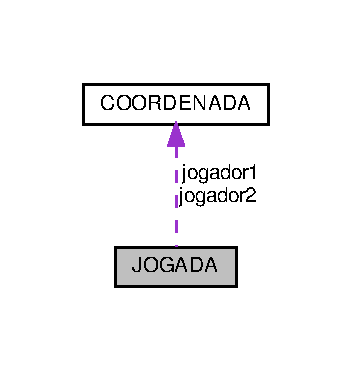
\includegraphics[width=169pt]{structJOGADA__coll__graph}
\end{center}
\end{figure}
\subsection*{Public Attributes}
\begin{DoxyCompactItemize}
\item 
\hyperlink{structCOORDENADA}{C\+O\+O\+R\+D\+E\+N\+A\+DA} \hyperlink{structJOGADA_a93d9306cb0c49b66b7d9a615bffe0149}{jogador1}
\item 
\hyperlink{structCOORDENADA}{C\+O\+O\+R\+D\+E\+N\+A\+DA} \hyperlink{structJOGADA_ab46b16dfbdc7f2af9430c8dcdac0914b}{jogador2}
\end{DoxyCompactItemize}


\subsection{Detailed Description}
Typedef no qual busca quais as coordenas que o jogador 1 ou jogador 2. 

\subsection{Member Data Documentation}
\mbox{\Hypertarget{structJOGADA_a93d9306cb0c49b66b7d9a615bffe0149}\label{structJOGADA_a93d9306cb0c49b66b7d9a615bffe0149}} 
\index{J\+O\+G\+A\+DA@{J\+O\+G\+A\+DA}!jogador1@{jogador1}}
\index{jogador1@{jogador1}!J\+O\+G\+A\+DA@{J\+O\+G\+A\+DA}}
\subsubsection{\texorpdfstring{jogador1}{jogador1}}
{\footnotesize\ttfamily \hyperlink{structCOORDENADA}{C\+O\+O\+R\+D\+E\+N\+A\+DA} J\+O\+G\+A\+D\+A\+::jogador1}

Coordenada do jogador 1 \mbox{\Hypertarget{structJOGADA_ab46b16dfbdc7f2af9430c8dcdac0914b}\label{structJOGADA_ab46b16dfbdc7f2af9430c8dcdac0914b}} 
\index{J\+O\+G\+A\+DA@{J\+O\+G\+A\+DA}!jogador2@{jogador2}}
\index{jogador2@{jogador2}!J\+O\+G\+A\+DA@{J\+O\+G\+A\+DA}}
\subsubsection{\texorpdfstring{jogador2}{jogador2}}
{\footnotesize\ttfamily \hyperlink{structCOORDENADA}{C\+O\+O\+R\+D\+E\+N\+A\+DA} J\+O\+G\+A\+D\+A\+::jogador2}

Coordenada do jogador 2 

The documentation for this struct was generated from the following file\+:\begin{DoxyCompactItemize}
\item 
camada\+De\+Dados.\+h\end{DoxyCompactItemize}

\hypertarget{structlista}{}\section{lista Struct Reference}
\label{structlista}\index{lista@{lista}}


Struct de lista ligada generalizada, ou seja, com void.  




{\ttfamily \#include $<$lista.\+h$>$}



Collaboration diagram for lista\+:\nopagebreak
\begin{figure}[H]
\begin{center}
\leavevmode
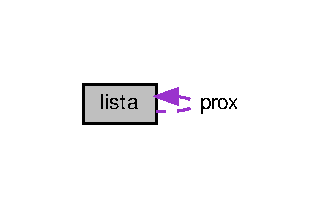
\includegraphics[width=155pt]{structlista__coll__graph}
\end{center}
\end{figure}
\subsection*{Public Attributes}
\begin{DoxyCompactItemize}
\item 
\mbox{\Hypertarget{structlista_a1851230b0237deef0519ee33de9f2dd0}\label{structlista_a1851230b0237deef0519ee33de9f2dd0}} 
void $\ast$ {\bfseries valor}
\item 
\mbox{\Hypertarget{structlista_a3b0e375147c1163d74544fd206a1f1de}\label{structlista_a3b0e375147c1163d74544fd206a1f1de}} 
struct \hyperlink{structlista}{lista} $\ast$ {\bfseries prox}
\end{DoxyCompactItemize}


\subsection{Detailed Description}
Struct de lista ligada generalizada, ou seja, com void. 

The documentation for this struct was generated from the following file\+:\begin{DoxyCompactItemize}
\item 
lista.\+h\end{DoxyCompactItemize}

%--- End generated contents ---

% Index
\backmatter
\newpage
\phantomsection
\clearemptydoublepage
\addcontentsline{toc}{chapter}{Index}
\printindex

\end{document}
